% ===================================================================
%  Week 7 — Lecture Notes (Persian) — Morphological Processing
% ===================================================================
\documentclass[12pt,a4paper]{article}
% ===================================================================
%  Shared preamble for Persian lecture notes (Image Processing).
%  Compile with XeLaTeX.  Body = Persian (RTL), code/math = LTR.
% ===================================================================

\usepackage{geometry}
\geometry{a4paper,margin=2.4cm}
\usepackage{amsmath,amssymb}
\usepackage{graphicx}
\usepackage{xcolor}
\usepackage{listings}
\usepackage{tcolorbox}
\usepackage{booktabs}
\usepackage{array}
\usepackage{enumitem}
\usepackage{hyperref}
\tcbuselibrary{skins,breakable}

% ---- Persian / RTL --------------------------------------------------
\usepackage{xepersian}
\settextfont{IRNazli}
\setlatintextfont{Latin Modern Roman}
\setdigitfont{IRNazli}
% More generous leading + paragraph spacing (Persian reads better with air).
\linespread{1.5}
\setlength{\parskip}{0.7em}

% ---- Colours --------------------------------------------------------
\definecolor{coursePrimary}{HTML}{1B4965}
\definecolor{courseAccent}{HTML}{E76F51}
\definecolor{courseGood}{HTML}{2A9D8F}
\definecolor{courseBad}{HTML}{C0392B}
\definecolor{courseInfo}{HTML}{2980B9}
\definecolor{codeBg}{HTML}{F5F6FA}
\definecolor{codeKw}{HTML}{8E44AD}
\definecolor{codeStr}{HTML}{2A9D8F}
\definecolor{codeCom}{HTML}{7F8C8D}

\hypersetup{colorlinks=true,linkcolor=courseInfo,urlcolor=courseInfo,citecolor=courseInfo}

% ---- Code listings (Python built in) -------------------------------
\lstdefinestyle{course}{
  backgroundcolor=\color{codeBg},
  basicstyle=\ttfamily\small,
  keywordstyle=\color{codeKw}\bfseries,
  stringstyle=\color{codeStr},
  commentstyle=\color{codeCom}\itshape,
  numberstyle=\tiny\color{codeCom},
  numbers=left, numbersep=7pt,
  showstringspaces=false, breaklines=true,
  tabsize=4, columns=fullflexible, frame=single,
  rulecolor=\color{gray!30}, keepspaces=true, upquote=true, language=Python,
}
\lstset{style=course}
\lstdefinelanguage{bash}{
  keywords={cd,pip,python,venv,source,import}, sensitive=true,
  morecomment=[l]{\#}, morestring=[b]', morestring=[b]",
}
\newenvironment{ltrcode}{\begin{LTR}}{\end{LTR}}

% ---- Callout boxes (Persian titles) --------------------------------
\newtcolorbox{yaddasht}{colback=courseInfo!8,colframe=courseInfo,
  title={\textbf{یادداشت}},boxrule=0.6pt,right=6pt,left=6pt,breakable}
\newtcolorbox{nokte}{colback=courseAccent!10,colframe=courseAccent,
  title={\textbf{نکتهٔ کلیدی}},boxrule=0.6pt,right=6pt,left=6pt,breakable}
\newtcolorbox{hoshdar}{colback=courseBad!8,colframe=courseBad,
  title={\textbf{هشدار / دام}},boxrule=0.6pt,right=6pt,left=6pt,breakable}
\newtcolorbox{riyazi}{colback=coursePrimary!6,colframe=coursePrimary,
  title={\textbf{ریاضیات}},boxrule=0.6pt,right=6pt,left=6pt,breakable}
\newtcolorbox{tamrin}{colback=courseGood!8,colframe=courseGood,
  title={\textbf{تمرین}},boxrule=0.6pt,right=6pt,left=6pt,breakable}

% ---- Header helper --------------------------------------------------
\newcommand{\coursemeta}[2]{%
  \begin{center}
  {\large\textbf{پردازش تصویرِ کاربردی}}\\[2pt]
  {\color{coursePrimary}\rule{\linewidth}{1pt}}\\[4pt]
  {\Large\textbf{#1}}\\[3pt]
  {\small جزوهٔ درس — #2}
  \end{center}\vspace{4pt}
}


\begin{document}
\coursemeta{جلسهٔ ۷ — پردازشِ مورفولوژیک}{هفتهٔ هفتم}

{\small\itshape مکملِ اسلایدهای انگلیسیِ جلسهٔ ۷. تصاویر از باینریِ واقعیِ کنتورِ شما تولید شده‌اند. هدف: شکل‌دادن، رشد، کوچک‌کردن و پاک‌سازیِ شکل‌های باینری با «عنصرِ ساختاری».}

\vspace{0.5cm}
\tableofcontents
\vspace{1cm}

% ===================================================================
\section{چرا این جلسه}

آستانه‌گذاری (جلسهٔ ۲) یک تصویرِ \textbf{باینری} می‌دهد — اما به‌هم‌ریخته (لکه، شکاف، ارقامِ شکسته).
امروز \textbf{مورفولوژی} را یاد می‌گیریم: عملیاتی که با یک \textbf{عنصرِ ساختاری} (\lr{SE}) شکل‌های
باینری را رشد، کوچک و تمیز می‌کنند. برای DocScan: پس از آستانه‌گذاریِ ارقام، مورفولوژی نویز را حذف
و شکاف‌ها را پُر می‌کند تا هر رقم یک لکهٔ تمیز و جداشدنی شود.

\begin{nokte}
مورفولوژی جراحیِ شکل است، نه هموارسازی. برخلافِ تاری که همه‌چیز را نرم می‌کند، مورفولوژی دربارهٔ
\emph{شکل} استدلال می‌کند و لبه‌ها را تیز نگه می‌دارد. ابزارِ درست پس از داشتنِ یک ماسکِ باینری است.
\end{nokte}

\subsection{مورفولوژی یعنی چه؟}

«مورفولوژی» یعنی «مطالعهٔ شکل». مورفولوژیِ ریاضی (که در دههٔ ۱۹۶۰ توسعه یافت) مجموعه‌ای از عملیات
برای تحلیل و پردازشِ \emph{شکل}‌های هندسیِ درونِ تصویر است. برخلافِ فیلترهای مکانی که با شدت کار
می‌کنند، مورفولوژی با \emph{ساختار} کار می‌کند: آیا این شکل به اندازهٔ کافی بزرگ است؟ آیا این
دو قطعه به هم متصل‌اند؟ آیا این سوراخ می‌تواند پُر شود؟

پایهٔ نظری‌اش نظریهٔ مجموعه‌هاست: تصویرِ باینری را مجموعه‌ای از نقاطِ سفید در نظر بگیرید، و عملیات
را به‌صورتِ عملیاتِ مجموعه‌ای (اجتماع، اشتراک، انتقال) روی آن. برای همین نمادهای $\oplus$ و
$\ominus$ (که شبیهِ جمع و تفریق‌اند) به کار می‌روند.

\begin{yaddasht}
شهودِ کلیدی: مورفولوژی تصویر را با یک «کاوشگر» (عنصرِ ساختاری) لمس می‌کند و می‌پرسد این کاوشگر
چطور با شکل‌ها تعامل می‌کند. تغییرِ کاوشگر (شکل و اندازه‌اش)، عملیاتِ متفاوتی می‌سازد — درست مثلِ
اینکه در جلسهٔ ۳ تغییرِ کرنل، فیلترِ متفاوتی می‌ساخت.
\end{yaddasht}

% ===================================================================
\section{دو عملیاتِ پایه}

\subsection{عنصرِ ساختاری}

یک شکلِ کوچک (\lr{SE}/کرنل) که روی تصویرِ باینری می‌لغزد — مثلِ یک کاوشگر. شکل‌های رایج: مستطیل،
بیضی، صلیب. \textbf{اندازه‌اش} تعیین می‌کند اثر چقدر تهاجمی است. مورفولوژی می‌پرسد: آیا SE اینجا
\emph{جا می‌شود} (فرسایش) یا \emph{برخورد می‌کند} (اتساع)؟

\begin{ltrcode}
\begin{lstlisting}[language=Python]
k = cv2.getStructuringElement(cv2.MORPH_ELLIPSE, (3, 3))  # 3x3 elliptical probe
\end{lstlisting}
\end{ltrcode}

\subsection{فرسایش و اتساع — روی ارقامِ واقعی}

\begin{center}

\includegraphics[width=0.31\linewidth]{../assets/binary.png}\quad

\includegraphics[width=0.31\linewidth]{../assets/erode.png}\quad

\includegraphics[width=0.31\linewidth]{../assets/dilate.png}\\[2pt]
{\small چپ: باینری — وسط: فرسایش (نازک‌تر) — راست: اتساع (ضخیم‌تر)}
\end{center}

\begin{itemize}
  \item \textbf{فرسایش} (\lr{erosion}): پیکسل را فقط اگر SE کاملاً درونِ شکل جا شود نگه می‌دارد $\rightarrow$ کوچک می‌شود، بخش‌های نازک را حذف می‌کند.
  \item \textbf{اتساع} (\lr{dilation}): پیکسل را اگر SE شکل را لمس کند ست می‌کند $\rightarrow$ رشد می‌کند، سوراخ‌های کوچک را پُر می‌کند.
\end{itemize}

\begin{riyazi}
فرسایش: $A \ominus B = \{z : B_z \subseteq A\}$ (SE کاملاً درونِ شکل).
اتساع: $A \oplus B = \{z : B_z \cap A \neq \emptyset\}$ (SE شکل را لمس می‌کند).
\end{riyazi}

\subsection{مثالِ عددیِ فرسایش}

بیایید فرسایش را با یک SEِ $3\times3$ (همه ۱) روی یک شکلِ کوچک ببینیم. فرسایش می‌گوید: یک پیکسل
سفید می‌ماند فقط اگر \emph{همهٔ} ۹ همسایه‌اش (شاملِ خودش) سفید باشند. برای یک خطِ سفیدِ نازک
(عرضِ ۱ پیکسل)، هیچ پیکسلی این شرط را ندارد (بالا و پایینش سیاه است)، پس خط کاملاً ناپدید می‌شود.
برای یک بلوکِ توپُر، فقط لبهٔ بیرونی حذف می‌شود و مغز می‌ماند. این توضیح می‌دهد چرا فرسایش
«جزئیاتِ نازک را حذف و شکل را کوچک می‌کند».

اتساع دقیقاً برعکس است: یک پیکسل سفید می‌شود اگر \emph{هر یک} از همسایه‌هایش سفید باشد. پس یک نقطهٔ
سفیدِ منفرد به یک بلوکِ $3\times3$ رشد می‌کند، و شکاف‌های باریک پُر می‌شوند.

\begin{nokte}
همین منطق «همه» در برابرِ «هر یک» تفاوتِ بنیادیِ فرسایش و اتساع است. فرسایش سخت‌گیر است (همه باید
سفید باشند)، اتساع سخاوتمند (یکی کافی است). ترکیبِ این دو (باز/بستن) قدرتِ واقعیِ مورفولوژی است.
\end{nokte}

\subsection{فرسایش و اتساع دوگان‌اند}

اتساعِ جلو‌زمینه = فرسایشِ پس‌زمینه (و برعکس). فرسایش حذف می‌کند: برجستگی‌های نازک، اشیای کوچک، و
اشیای متصل را \textbf{جدا} می‌کند. اتساع اضافه می‌کند: شکاف‌ها را پُر می‌کند، قطعاتِ نزدیک را
وصل می‌کند، و ضربه‌های نازک را \textbf{ضخیم} می‌کند.

\begin{hoshdar}
هرکدام تحریف هم می‌کنند: فرسایش می‌تواند یک رقمِ نازک را بشکند؛ اتساع می‌تواند دو رقمِ نزدیک را
ادغام کند. اندازهٔ SE مهم است.
\end{hoshdar}

% ===================================================================
\section{باز و بسته کردن (Opening \& Closing)}

\subsection{باز کردن = فرسایش سپس اتساع}

\begin{center}

\includegraphics[width=0.44\linewidth]{../assets/noisy.png}\quad

\includegraphics[width=0.44\linewidth]{../assets/open.png}\\[2pt]
{\small چپ: باینری + لکه — راست: باز کردن (لکه‌ها حذف)}
\end{center}

\textbf{باز کردن} (\lr{opening}) لکه‌های روشنِ کوچک را حذف می‌کند در حالی که اندازهٔ ارقام را نگه
می‌دارد (فرسایش آن‌ها را می‌کشد، اتساع بقیه را بازمی‌گرداند). عملیاتِ کلاسیکِ «پاک‌سازیِ نویزِ نمک
روی یک ماسکِ باینری».

\subsection{بستن = اتساع سپس فرسایش}

\begin{center}

\includegraphics[width=0.44\linewidth]{../assets/binary.png}\quad

\includegraphics[width=0.44\linewidth]{../assets/close.png}\\[2pt]
{\small چپ: باینری — راست: بستن (شکاف‌ها پُر شد)}
\end{center}

\textbf{بستن} (\lr{closing}) سوراخ‌ها و شکاف‌های کوچکِ درونِ شکل‌ها را پُر می‌کند در حالی که اندازه
را نگه می‌دارد. یک رقمی را که آستانه‌گذاری شکسته، به یک ضربهٔ توپُر ترمیم می‌کند.

\begin{center}
\begin{tabular}{>{\raggedright\arraybackslash}p{0.2\linewidth} >{\raggedright\arraybackslash}p{0.28\linewidth} >{\raggedright\arraybackslash}p{0.42\linewidth}}
\toprule
\textbf{عملیات} & \textbf{ترتیب} & \textbf{اثر} \\
\midrule
باز کردن & فرسایش $\rightarrow$ اتساع & حذفِ لکه‌های \emph{روشن}، شکستنِ اتصالِ نازک \\
بستن & اتساع $\rightarrow$ فرسایش & پُرکردنِ سوراخ‌های \emph{تاریک}، پل‌زدنِ شکاف \\
\bottomrule
\end{tabular}
\end{center}

\begin{nokte}
باز کردن بیرون را تمیز می‌کند؛ بستن درون را ترمیم می‌کند. هر دو اندازهٔ کلی را نگه می‌دارند،
برخلافِ فرسایش/اتساعِ خام. برای همین در پاک‌سازیِ ماسک از این دو استفاده می‌کنیم، نه از فرسایش/اتساعِ تنها.
\end{nokte}

\subsection{چرا ترتیب مهم است}

باز کردن = فرسایش سپس اتساع. چرا این ترتیب لکه را حذف می‌کند اما ارقام را نگه می‌دارد؟ گامِ اولِ
\emph{فرسایش} هم لکه‌های کوچک و هم لبهٔ بیرونیِ ارقام را می‌خورد؛ لکه‌های کوچک کاملاً ناپدید
می‌شوند اما ارقام (بزرگ‌تر) فقط کمی کوچک می‌شوند. گامِ دومِ \emph{اتساع} لبهٔ خورده‌شدهٔ ارقام را
بازمی‌گرداند — اما چیزی برای بازگرداندنِ لکه‌ها نمانده. نتیجه: ارقام با اندازهٔ اصلی، بدونِ لکه.

بستن برعکس است: اتساع اول شکاف‌ها را پُر و ارقام را کمی بزرگ می‌کند؛ فرسایشِ بعدی اندازه را
بازمی‌گرداند اما شکافِ پُرشده باقی می‌ماند. این تقارنِ زیبا توضیح می‌دهد چرا این دو عملیات
«حفظ‌کنندهٔ اندازه» هستند در حالی که فرسایش/اتساعِ خام نیستند.

\begin{riyazi}
باز کردن: $A \circ B = (A \ominus B) \oplus B$. \quad بستن: $A \bullet B = (A \oplus B) \ominus B$.
یک خاصیتِ مهم: باز/بستن \textbf{خودتوان} (\lr{idempotent}) هستند — اعمالِ دوباره‌شان چیزی را تغییر
نمی‌دهد. یعنی $(A \circ B) \circ B = A \circ B$.
\end{riyazi}

\subsection{کدام عملیات برای کدام نقص}

\begin{center}
\begin{tabular}{>{\raggedright\arraybackslash}p{0.42\linewidth} >{\raggedright\arraybackslash}p{0.48\linewidth}}
\toprule
\textbf{نقص در ماسکِ باینری} & \textbf{عملیات} \\
\midrule
لکه‌های سفیدِ کوچک (نمک) & باز کردن \\
سوراخ‌های سیاهِ کوچک درونِ شکل & بستن \\
شکافِ باریک در یک ضربه & بستن \\
دو شیء که با یک پلِ نازک وصل‌اند & باز کردن (پل را می‌شکند) \\
شیء کمی بزرگ‌تر از نیاز & فرسایش \\
شیء کمی کوچک‌تر از نیاز & اتساع \\
نیاز به طرحِ کلی & گرادیانِ مورفولوژیک \\
پس‌زمینهٔ ناهموار & top-hat (روی خاکستری) \\
\bottomrule
\end{tabular}
\end{center}

این جدول را کنارِ دست داشته باشید: پاک‌سازیِ ماسک عمدتاً تطبیقِ نقص با عملیاتِ درست است.

% ===================================================================
\section{عملیاتِ بیشتر}

\begin{center}
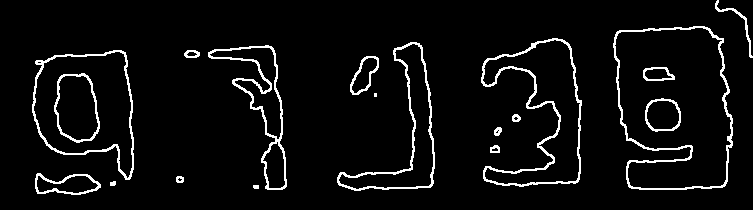
\includegraphics[width=0.5\linewidth]{../assets/gradient.png}\\[2pt]{\small گرادیانِ مورفولوژیک = طرحِ کلی}
\end{center}

\begin{itemize}
  \item \textbf{گرادیان} = اتساع $-$ فرسایش $\rightarrow$ طرحِ کلیِ شیء.
  \item \textbf{بالاسیلندری} (\lr{top-hat}) = تصویر $-$ باز کردن $\rightarrow$ جزئیاتِ روشنِ کوچک (تصحیحِ نورِ ناهموار!).
  \item \textbf{سیاه‌سیلندری} (\lr{black-hat}) = بستن $-$ تصویر $\rightarrow$ جزئیاتِ تاریکِ کوچک.
\end{itemize}

\begin{yaddasht}
\lr{top-hat} یک رفعِ نور است: ارقام را از یک پس‌زمینهٔ آرام‌تغییر جدا می‌کند. اگر یک عکسِ کنتور
سایه‌ای در بخشی دارد، \lr{top-hat} می‌تواند آن را یکنواخت کند پیش از آستانه‌گذاری — یک ترفندِ قدرتمندِ DocScan.
\end{yaddasht}

\subsection{top-hat با جزئیات: چرا نور را تصحیح می‌کند}

\lr{top-hat} = تصویر منهای باز‌شدهٔ آن. چرا این نورِ ناهموار را رفع می‌کند؟ باز کردن با یک SEِ بزرگ،
ساختارهای \emph{بزرگ‌تر از SE} (مثلِ پس‌زمینهٔ آرام‌تغییر و نور) را نگه می‌دارد و کوچک‌ترها (مثلِ
ارقام) را حذف می‌کند. پس «باز‌شده» تقریباً همان پس‌زمینهٔ نوری است. تفریقِ آن از تصویرِ اصلی، فقط
ساختارهای کوچک (ارقام) را باقی می‌گذارد — روی یک زمینهٔ یکنواخت.

مثال: یک عکسِ کنتور که یک گوشه‌اش تاریک است. آستانه‌گذاریِ مستقیم شکست می‌خورد (یک آستانهٔ واحد
برای هر دو ناحیه کار نمی‌کند). اما پس از top-hat، پس‌زمینه یکنواخت می‌شود و یک آستانهٔ ساده کار
می‌کند. این جایگزینِ قدرتمندی برای آستانه‌گذاریِ تطبیقی است.

\begin{riyazi}
\lr{top-hat}: $T(f) = f - (f \circ B)$. \quad \lr{black-hat}: $B(f) = (f \bullet B) - f$.
اولی جزئیاتِ روشن‌تر از محیط، دومی تاریک‌تر از محیط را جدا می‌کند.
\end{riyazi}

\subsection{مورفولوژیِ خاکستری}

مورفولوژی روی خاکستری هم کار می‌کند: فرسایش = کمینهٔ محلی، اتساع = بیشینهٔ محلی. \lr{top-hat} روی
خاکستری یک گرادیانِ نرمِ پس‌زمینه را حذف می‌کند — عالی پیش از آستانه‌گذاری. پس مورفولوژی فقط برای
باینری نیست — یک ابزارِ عمومیِ شکل/شدت است.

% ===================================================================
\section{تمرینِ کلاسیِ وسط‌جلسه (۱۲ دقیقه)}

\begin{tamrin}
کنتورِ آستانه‌گذاری‌شدهٔ شما این مشکلات را دارد. کدام مورفولوژی هرکدام را رفع می‌کند؟ (۱) پیکسل‌های
سفیدِ منفردِ پراکنده (نمک) دورِ ارقام. (۲) یک رقم توسطِ شکافِ آستانه به دو تکه شکسته. (۳) دو رقمِ
مجاور به هم چسبیده‌اند و باید برای شمارش جدا شوند. (۴) فقط طرحِ کلیِ هر رقم را می‌خواهید.
\end{tamrin}

\textbf{جمع‌بندی:} (۱) لکه‌های نمک $\rightarrow$ \textbf{باز کردن} (SE کوچک). (۲) رقمِ شکسته
$\rightarrow$ \textbf{بستن}. (۳) ارقامِ چسبیده $\rightarrow$ \textbf{فرسایش} (با احتیاط) برای جدا
کردن، یا \lr{watershed} (جلسهٔ ۸). (۴) طرحِ کلی $\rightarrow$ \textbf{گرادیانِ مورفولوژیک}. نقص را
تشخیص دهید (لکه/شکاف/ادغام)، بعد عملیات و اندازهٔ SE متناظر را انتخاب کنید.

% ===================================================================
\section{بخشِ عمیق}

\subsection{شکل و اندازهٔ عنصرِ ساختاری}

SEِ بزرگ‌تر = اثرِ قوی‌تر (حذفِ لکه‌های بزرگ‌تر / پُرکردنِ شکاف‌های بزرگ‌تر) اما تحریفِ بیشتر. شکل
مهم است: یک SEِ عمودی روی ضربه‌های عمودی متفاوت از افقی اثر می‌گذارد. قاعده: \emph{کوچک‌ترین}
SEی را که نقص را رفع کند به کار ببرید — بزرگ‌تر جزئیاتِ واقعی را پاک می‌کند.

\begin{center}
\begin{tabular}{>{\raggedright\arraybackslash}p{0.22\linewidth} >{\raggedright\arraybackslash}p{0.28\linewidth} >{\raggedright\arraybackslash}p{0.42\linewidth}}
\toprule
\textbf{شکلِ SE} & \textbf{کِی} & \textbf{نکته} \\
\midrule
مستطیل & پاک‌سازیِ عمومی & سریع، اثرِ مربعی \\
بیضی & اشیای گرد & نرم‌تر، طبیعی‌تر \\
صلیب & اتصال‌های نازک & کمینه، ملایم \\
خط (افقی/عمودی) & جهت‌دار & حذف/حفظِ ضربه‌های افقی یا عمودی \\
\bottomrule
\end{tabular}
\end{center}

\begin{hoshdar}
یک SEِ خیلی بزرگ ارقام را به لکه‌های ناشناختنی تبدیل می‌کند. اندازه را روی دادهٔ واقعی تنظیم کنید.
\end{hoshdar}

\subsection{حذفِ خط، حفظِ متن}

یک فرم ضربه‌های جدول/زیرخط دارد که می‌خواهید بروند اما متن بماند. از یک SEِ خطیِ \emph{افقیِ} بلند
با باز کردن استفاده کنید تا خطوطِ افقی را جدا کنید، سپس تفریقشان کنید. یک SEِ جهت‌دار ابزارِ دقیقی
است — فقط روی ساختارهایی با جهت و طولِ انتخابی عمل می‌کند. برای یک فرمِ اسکن‌شده (موردِ DocScan)،
این خطوط/جعبه‌ها را از محتوای دست‌نویس تمیز جدا می‌کند.

\subsection{بازسازیِ مورفولوژیک}

یک تکنیکِ پیشرفته و بسیار مفید: \textbf{بازسازی} (\lr{morphological reconstruction}). به‌جای یک
باز کردنِ ساده که شکل را کمی تغییر می‌دهد، بازسازی از یک «نشانگر» شروع می‌کند و آن را زیرِ یک
«ماسک» به‌طورِ مکرر اتساع می‌دهد تا پایدار شود. نتیجه: اشیایی که نشانگر آن‌ها را لمس می‌کند
\emph{کاملاً و با شکلِ اصلی} بازیابی می‌شوند، و بقیه حذف می‌شوند.

کاربردِ عملی: «همهٔ ارقامی را نگه دار که به لبهٔ تصویر نمی‌رسند» یا «همهٔ اشیایی را حذف کن که از
یک اندازهٔ خاص کوچک‌ترند، بدونِ تغییرِ شکلِ بقیه». برخلافِ باز کردن که لبه‌ها را کمی تغییر می‌دهد،
بازسازی شکل‌ها را دست‌نخورده نگه می‌دارد — فقط انتخاب می‌کند کدام بمانند.

\begin{yaddasht}
بازسازی نشان می‌دهد که مورفولوژی فراتر از چهار عملیاتِ پایه است. با ترکیبِ هوشمندانهٔ فرسایش و
اتساعِ شرطی، می‌توان عملیاتِ بسیار قدرتمندی ساخت که در پاک‌سازیِ دقیقِ ماسک (مثلِ DocScan) بی‌نظیرند.
\end{yaddasht}

\subsection{اسکلت‌سازی و نازک‌سازی}

\textbf{اسکلت}: یک شکل را مکرراً نازک کنید تا به یک «ستون فقرات»ِ تک‌پیکسلی برسد — جوهرِ توپولوژیکش.
مفید برای تحلیلِ کاراکتر/ضربه و اندازه‌گیریِ اتصال. مرتبط: \textbf{برخورد-یا-عدمِ‌برخورد}
(\lr{hit-or-miss}) الگوهای محلیِ دقیق (گوشه، نقطهٔ پایانی) را می‌یابد.

\subsection{گرانولومتری: اندازه‌گیریِ اندازه‌ها}

یک کاربردِ زیبا: با باز کردنِ مکرر با SEهای بزرگ‌ترِ متوالی و شمردنِ پیکسل‌های باقی‌مانده، می‌توانید
\textbf{توزیعِ اندازهٔ} اشیا را اندازه بگیرید (\lr{granulometry}). اشیای کوچک‌تر از SE با هر گام
حذف می‌شوند، پس افتِ ناگهانی در تعدادِ پیکسل نشان‌دهندهٔ اندازهٔ غالبِ اشیاست. این در تحلیلِ
سلول‌ها، دانه‌ها، یا حباب‌ها به کار می‌رود — بدونِ نیاز به قطعه‌بندیِ صریح.

\begin{yaddasht}
گرانولومتری نمونه‌ای از تفکرِ مورفولوژیک است: به‌جای «هر شیء را جدا کن و اندازه بگیر»، از خودِ
عملیاتِ مورفولوژیک برای استخراجِ آمارِ اندازه استفاده می‌کنید. اغلب ساده‌تر و مقاوم‌تر از قطعه‌بندیِ کامل است.
\end{yaddasht}

\subsection{استخراجِ مرز و پُرکردنِ سوراخ}

\textbf{مرز} = تصویر $-$ فرسایش (یک طرحِ کلیِ نازک؛ مقایسه با گرادیانِ مورفولوژیک).
\textbf{پُرکردنِ سوراخ}: نواحیِ تاریکِ محصور درونِ یک شکل را پُر می‌کند (یک رقمِ توپُر از یک توخالی).
این‌ها روی فرسایش/اتساع ساخته می‌شوند — مورفولوژی یک جعبه‌ابزارِ کوچک است که به بسیاری اثرها ترکیب می‌شود.

% ===================================================================
\section{کارایی و پیاده‌سازی}

مورفولوژی می‌تواند گران باشد اگر ساده پیاده شود، اما چند ترفند آن را سریع می‌کند:

\begin{itemize}
  \item \textbf{تفکیک‌پذیری}: یک SEِ مستطیلیِ $k\times k$ = یک SEِ افقیِ $1\times k$ سپس یک عمودیِ $k\times 1$ — بسیار سریع‌تر.
  \item \textbf{تکرار}: فرسایشِ با SEِ $3\times3$ دوبار $\approx$ فرسایش با SEِ $5\times5$ یک‌بار — گاهی ارزان‌تر.
  \item \lr{OpenCV} این بهینه‌سازی‌ها را خودکار انجام می‌دهد؛ شما فقط عملیات و SE را مشخص کنید.
\end{itemize}

\begin{nokte}
برای تصاویرِ بزرگ (مثلِ یک صفحهٔ اسکن‌شدهٔ کامل)، انتخابِ اندازه و شکلِ SE هم بر کیفیت و هم بر
سرعت اثر می‌گذارد. یک SEِ کوچکِ تکرارشده اغلب از یک SEِ بزرگِ واحد هم سریع‌تر و هم قابلِ‌کنترل‌تر است.
\end{nokte}

% ===================================================================
\section{این جلسه در پروژهٔ نهایی}

ترتیبِ نوعیِ DocScan: آستانه $\rightarrow$ باز کردن (حذفِ نویز) $\rightarrow$ بستن (ترمیمِ ارقام)
$\rightarrow$ کانتور (جلسهٔ ۹). ترتیب مهم است: باز کردن پیش از بستن مانعِ ادغامِ یک لکه در یک رقم
می‌شود.

\begin{ltrcode}
\begin{lstlisting}[language=Python]
_, b = cv2.threshold(gray, 0, 255, cv2.THRESH_BINARY_INV + cv2.THRESH_OTSU)
k = cv2.getStructuringElement(cv2.MORPH_ELLIPSE, (3, 3))
clean = cv2.morphologyEx(b, cv2.MORPH_OPEN, k)    # remove specks
clean = cv2.morphologyEx(clean, cv2.MORPH_CLOSE, k)  # repair digits
# next: find each digit's contour (Week 9)
\end{lstlisting}
\end{ltrcode}

\begin{yaddasht}
\textbf{مایلستونِ هفتهٔ ۷:} یک باینریِ تمیز تولید کنید که هر رقم یک لکهٔ توپُر و جداشدنی باشد. اگر
دو رقم چسبیده‌اند، فرسایشِ ملایم یا watershed (جلسهٔ ۸) لازم است. کیفیتِ این پاک‌سازی، مستقیماً
موفقیتِ شمارش و شناساییِ ارقام را تعیین می‌کند.
\end{yaddasht}

\subsection{پل به قطعه‌بندی (watershed)}

مورفولوژی پایهٔ برخی روش‌های قطعه‌بندیِ جلسهٔ ۸ است. مثال: برای جدا کردنِ اشیای چسبیده، ابتدا با
فرسایشِ مکرر «مرکز»ِ قطعیِ هر شیء را می‌یابید (نواحیِ پیش‌زمینهٔ قطعی)، سپس با اتساع نواحیِ
پس‌زمینهٔ قطعی را، و ناحیهٔ نامعلومِ بین آن‌ها را با \lr{watershed} تقسیم می‌کنید. پس مورفولوژیِ
امروز، مستقیماً ورودیِ قطعه‌بندیِ جلسهٔ ۸ را آماده می‌کند.

\begin{ltrcode}
\begin{lstlisting}[language=Python]
sure_fg = cv2.erode(binary, k, iterations=3)   # definite object centers
sure_bg = cv2.dilate(binary, k, iterations=3)  # definite background
unknown = cv2.subtract(sure_bg, sure_fg)       # the boundary region
# watershed uses these markers (Week 8)
\end{lstlisting}
\end{ltrcode}

\subsection{مورفولوژی در برابرِ تاری}

تاری میانگین می‌گیرد (همه‌چیز را نرم می‌کند)؛ مورفولوژی دربارهٔ \emph{شکل} استدلال می‌کند (لبه‌ها
را سخت نگه می‌دارد). برای حذفِ لکه از یک ماسکِ \emph{باینری}، باز کردن از تاری بهتر است (که آن را
خاکستری می‌کرد). تاری را روی خاکستری/نویز، مورفولوژی را روی شکل‌های باینری استفاده کنید.

% ===================================================================
\section{جمع‌بندی}

\begin{itemize}
  \item توضیحِ فرسایش/اتساع با عنصرِ ساختاری (جا شدن در برابرِ برخورد).
  \item استفاده از باز کردن (حذفِ لکه) و بستن (پُرکردنِ شکاف)؛ انتخابِ اندازهٔ SE.
  \item اعمالِ گرادیان/بالاسیلندری/سیاه‌سیلندری؛ تصحیحِ نورِ ناهموار با top-hat.
  \item ساختِ خطِ لولهٔ آستانه $\rightarrow$ پاک‌سازیِ مورفولوژیک برای ارقام.
\end{itemize}

\begin{tamrin}
\textbf{تحویلیِ این هفته (پیش از جلسهٔ ۸):} روی یک کنتور/پلاکِ آستانه‌گذاری‌شده (از جلسهٔ ۲):
(۱) فرسایش، اتساع، باز و بسته کردن را نمایش دهید؛ هر اثر را توضیح دهید. (۲) با باز کردن نویزِ
لکه‌ای و با بستن ارقامِ شکسته را رفع کنید. (۳) top-hat را روی عکسی با نورِ ناهموار اعمال کنید؛ با
قبل مقایسه کنید. (۴) مایلستونِ DocScan: یک باینریِ تمیز که هر رقم یک لکهٔ توپُر و جداشدنی است.
\end{tamrin}

\subsection*{کاربردهای مورفولوژی}

\begin{itemize}
  \item \textbf{پاک‌سازیِ ماسک}: حذفِ نویز و ترمیمِ شکل پس از آستانه (DocScan).
  \item \textbf{جداسازی/شمارش}: جدا کردنِ اشیای چسبیده پیش از شمارش.
  \item \textbf{استخراجِ ویژگی}: اسکلت، طرحِ کلی، گوشه‌ها برای تحلیلِ شکل.
  \item \textbf{تصحیحِ نور}: top-hat برای یکنواخت‌کردنِ پس‌زمینه.
  \item \textbf{حذفِ ساختار}: خطوطِ جدول، شبکه، پس‌زمینهٔ فرم.
\end{itemize}

\subsection*{چک‌لیستِ دام‌های این هفته}

\begin{itemize}
  \item SEِ خیلی بزرگ (نابودیِ ارقام) — کوچک‌ترین SEی که کار کند.
  \item ترتیبِ اشتباه (بستن پیش از باز کردن، ادغامِ لکه در رقم) — اول باز، بعد بسته.
  \item مورفولوژی روی تصویرِ غیرباینری بدونِ فکر — نتایجِ غیرمنتظره.
  \item فراموشیِ قراردادِ جلو‌زمینه (سفید=شیء) — عملیات معکوس عمل می‌کند.
  \item انتظارِ معجزه از مورفولوژی روی آستانه‌گذاریِ بد — اول آستانهٔ خوب.
\end{itemize}

\subsection*{واژه‌نامهٔ کوتاه}

\begin{center}
\begin{tabular}{>{\raggedright\arraybackslash}p{0.3\linewidth} >{\raggedright\arraybackslash}p{0.6\linewidth}}
\toprule
\textbf{اصطلاح} & \textbf{معنی} \\
\midrule
\lr{Structuring element} & کاوشگرِ کوچک که عملیات را تعریف می‌کند \\
\lr{Erosion / Dilation} & کوچک‌کردن / رشدِ شکل \\
\lr{Opening / Closing} & حذفِ لکه / پُرکردنِ شکاف \\
\lr{Top-hat} & جزئیاتِ روشنِ کوچک (تصحیحِ نور) \\
\lr{Gradient} & طرحِ کلیِ شکل (اتساع $-$ فرسایش) \\
\lr{Skeleton} & ستون فقراتِ تک‌پیکسلیِ شکل \\
\bottomrule
\end{tabular}
\end{center}

\vspace{0.5cm}
\begin{center}
\textit{آستانه آن را باینری می‌کند؛ مورفولوژی آن را تمیز می‌کند. باز کردن لکه‌ها را می‌برد، بستن شکاف‌ها را پُر می‌کند.}
\end{center}

\end{document}
